\chapter{Introduction}
\label{ch1}

%
The last decade has experienced a rapid growth in the world population, and, in the following years, the number of people it is expected to increase with a rate of $1.1\%$ for year, reaching $9.7$ billions by 2050 \cite{wpp}. As the world population increases, so the energy demand does.
% The increase of population has led to a rise of power demand that can not always be satisfied with non-renewable energy only.
This high energy demand has required an intensive usage of fossil energy, causing environmental pollution and changes in the climate.\\ 
Indeed, the increase of global temperature and the worsening of the air quality are posing a real problem for the environment. In the last years, some changes have been observed in Earth’s climate, primarily driven by human activities, particularly fossil fuel burning. \\

The biggest disadvantage of fossil fuels is that during the process of combustion in addition to energy, greenhouse gases (\gls{GHG}) are emitted \cite{greenhousegasemissions}. \\
These gases form a cope in the atmosphere, similar to glass in greenhouses, that traps the heat, increasing the Earth's temperature. \\
For around a century, humans have relied on fossil fuels, like oil, natural gas and coil for everyday tasks: heating, transportation and to produce electricity. For this reason, the \gls{GHG} emissions have reached historical peaks and are expected to increase in the following years \cite{co2predic}: in the year 2020, the concentration of \gls{CarbonDiox} in the atmosphere had risen to $48\%$ above its pre-industrial level (before 1750). \\

In order to improve the situation, the 2015 Paris Agreement set an ambition to limit global warming to well below $\SI{2}{\degreeCelsius}$ above pre-industrial levels and pursue efforts to limit it to $\SI{1.5}{\degreeCelsius}$ - in part by pursuing net carbon neutrality by 2050. The substantial reduction of global greenhouse gas emissions (including \gls{CarbonDiox})  would limit the increase of global temperature \cite{french_conference}. \\
Countries were asked to go through a process of decarbonisation: the reduction of carbon dioxide emissions through the use of low carbon power sources. \\
%Renewable energy production has low or no waste products such as \gls{CarbonDiox} or other chemical pollutants.  \\
% These low carbon power sources usually are renewable energies such as sun, wind, geothermal heat and other natural sources.
These sources convert the energy coming through naturals elements (sun, wind, geothermal heat) in another form of energy, electricity for example, with low or no waste products such as \gls{CarbonDiox} or other chemical pollutants. 

\begin{figure}[H]
\centering
    % 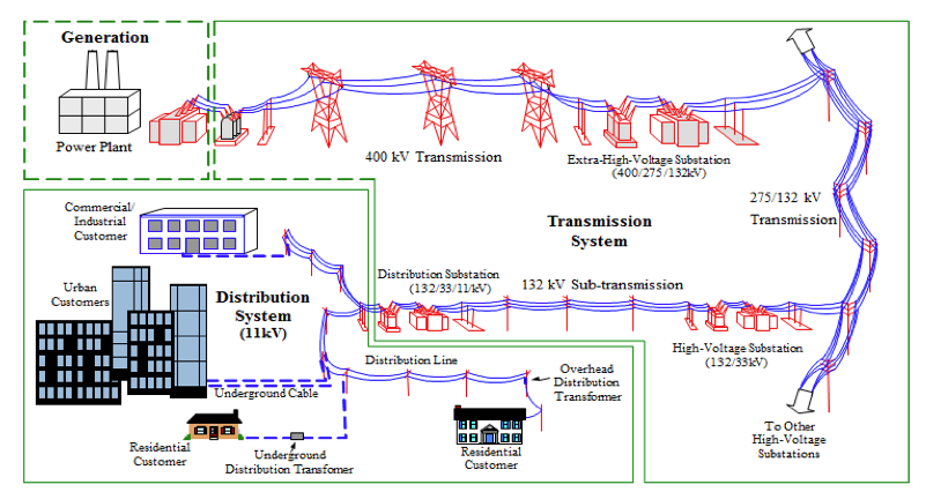
\includegraphics[width=.9\linewidth]{images/DN/HighMediumLowV.png}
    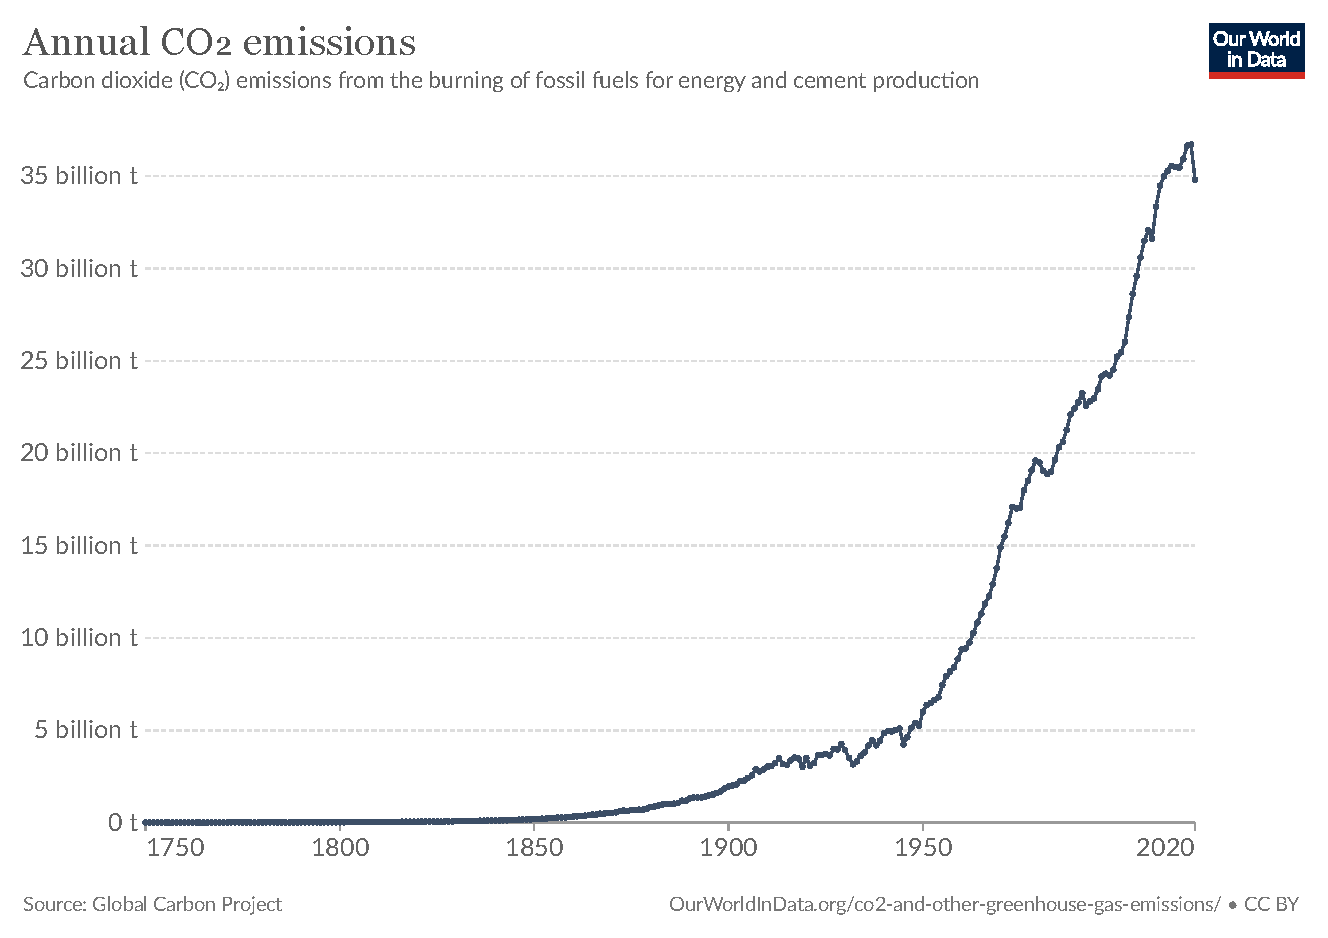
\includegraphics[width=.7\linewidth]{images/Introduction/annual-co2-emissions-per-country.pdf}
\caption[\gls{CarbonDiox} production over the years]{World \gls{CarbonDiox} production over the years \cite{C02prod}.}
\end{figure}

Thanks to this emerging trend of decarbonisation, more and more renewable power energy devices are introduced in the distribution networks \cite{owidenergy}. With the advantages of inexhaustibility and low impact on the environment, the high penetration of these renewables devices bring in some technical complications for the transmission and distribution of power in the grids. \\
The networks, that have been designed around the conventional centralized energy production, have to adapt to the new generators in the system. The distribution networks are moving from unidirectional power flow (from the distribution system to the consumers) to a bidirectional power flow (in this case the consumers are also producers and the exceed energy can be transported from the consumers to the distribution system. They are also known as prosumers \cite{prosumers}). This switch from unidirectional to bidirectional power flow requires a smarter system that can handle in an efficient way the generation and distribution of energy.\\

In the literature, this smarter way to control a power grid is known as active network management (\gls{ANM}) and it refers to the design of control schemes that control the distributed energy resources (\glspl{DER}), the loads, and the distributed energy storages (\glspl{DES}), as well as other elements like switches, connected to the grid. \\


% \noindent The time series from the Simbench database are fit to the Pandapower network and the power flow is calculated, obtaining all the information needed to build a database. This information is used to train a model to forecast the voltage problems and an agent that can control the network to solve these issues.

\section{Aim of the thesis}
The aim of this thesis is to exploit data-driven approaches to forecast and control the future nodes' voltage problems based on historical measurements in a medium-voltage distribution system using machine learning techniques, with a particular focus on deep artificial neural networks. The objectives of this thesis are to:
\begin{enumerate}[label=\textbf{\Roman*)}]
    \item \label{aim1}  Build a time series dataset that is used to train the machine learning models. A real medium-voltage network from the Pandapower python library is used. This network is fit with time series taken from the SimBench database, a database generated by the measurements of real loads and generators from Germany. 
    
    \item \label{aim2} Predict the voltage fluctuation problems in the network under a supervised learning framework. The three artificial neural networks used are: a multi layer perceptron, a convolutional neural network and a recurrent neural network. Three combinations of network information are tested, and some techniques for unbalanced datasets are examined as well. \\
    Different combinations are used since the network operator can have access to a limited amount of data, so the performances for each combination are reported.
    
    \item \label{aim3} Control the active and reactive power of the network's generators using reinforcement learning framework. The model used is a deep deterministic policy gradient algorithm that allows to work with continuos state and action space.\\
    The agent changes the generators' output in order to keep the voltage magnitude of the network's buses inside a safe voltage range.
\end{enumerate}
Predicting the contingency problems and controlling the network's devices would allow reducing possible consequences related to voltage issues, like for example over voltages problems. 
% Moreover, some control techniques are employed to avoid the network's critical situations.
% \begin{figure}[H]
% \centering
%     % 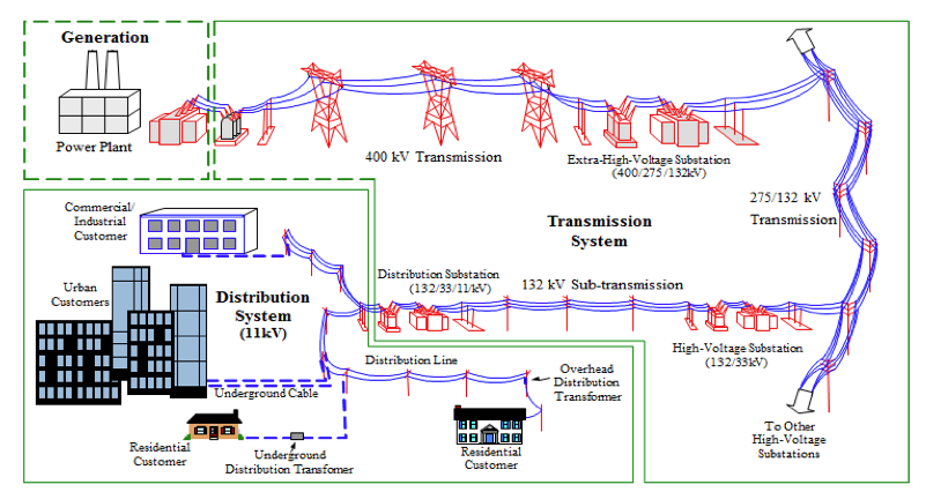
\includegraphics[width=.9\linewidth]{images/DN/HighMediumLowV.png}
%     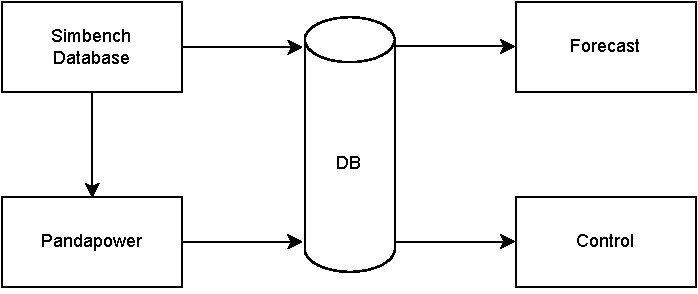
\includegraphics[width=.6\linewidth]{images/Introduction/Steps MT.pdf}
% \caption[Main steps of this master's thesis]{Main steps of this master's thesis}
% \end{figure}

\section{Thesis outline}

The document is organised into six chapters.\\ 

% \noindent In \textbf{chapter \ref{ch1}} it is presented  an introduction of the problem, presenting the literature review and the goals of the thesis.\\

\noindent \textbf{Chapter \ref{ch2}} provides the background information needed to understand this thesis's work, in particular in \ref{sec:2ps} it is presented a short description of how power networks work, an important calculation in power networks: the power flow; and some observations on voltage problems. In \ref{sec:2ml}, it is presented an overview of machine learning, with emphasis on artificial neural networks. In \ref{sec:sl} a description of the concepts of supervised learning, the models and evaluation metrics used in this thesis. Moreover, some techniques to handle unbalanced datasets are presented. \\
In \ref{sec:rl} a description of the concepts of reinforcement learning, a model and some evaluation metrics is presented.\\
After an introduction of the different terms and concepts, the literature review is proposed in \ref{sec:lr}.\\

\noindent \textbf{Chapter \ref{ch3}} provides the information about the use case studied. In particular, the description of the MV Oberrhein network is presented in \ref{sec:3mvon}, an overview of the SimBench database in \ref{sec:3sd} and how the time series are selected in \ref{sec:3tss}.\\

\noindent \textbf{Chapter \ref{ch4}} provides the main development of the project. The problem is defined in a rigorous way in \ref{sec:4ps}. In \ref{sec:4sm} the solving methodology is proposed with the description with the forecast of possible over voltage situations and the control the network's devices in order to avoid these situations.\\

\noindent \textbf{Chapter \ref{ch5}} provides the results of the different combinations of the forecasting part in \ref{sec:5fr} and of the controlling part in \ref{sec:5cr}. A discussion of the values obtained is presented as well.\\

\noindent The thesis ends with \textbf{chapter \ref{ch6}} that provides the conclusion and a discussion on some possible future works.


